% Created 2024-03-11 lun 20:21
% Intended LaTeX compiler: pdflatex
\documentclass[aspectratio=169, usenames,svgnames,dvipsnames]{beamer}
\usepackage[utf8]{inputenc}
\usepackage[T1]{fontenc}
\usepackage{graphicx}
\usepackage{longtable}
\usepackage{wrapfig}
\usepackage{rotating}
\usepackage[normalem]{ulem}
\usepackage{amsmath}
\usepackage{amssymb}
\usepackage{capt-of}
\usepackage{hyperref}
\usepackage{color}
\usepackage{listings}
\usepackage{mathpazo}
\usepackage{gensymb}
\usepackage{amsmath}
\usepackage{diffcoeff}
\usepackage{steinmetz}
\usepackage{mathtools}
\usepackage{fancyvrb}
\DefineVerbatimEnvironment{verbatim}{Verbatim}{fontsize=\tiny, formatcom = {\color{black!70}}}
\bibliographystyle{plain}
\usepackage{siunitx}
\sisetup{per-mode=symbol}
\sisetup{output-decimal-marker={,}}
\DeclareSIUnit{\watthour}{Wh}
\DeclareSIUnit{\wattpeak}{Wp}
\DeclareSIUnit{\watthour}{Wh}
\DeclareSIUnit{\amperehour}{Ah}
\usepackage{steinmetz}
\hypersetup{colorlinks=true, linkcolor=Blue, urlcolor=Blue}
\usepackage[symbol, perpage]{footmisc}
\parskip=5pt
\usetheme{Boadilla}
\usecolortheme{rose}
\usefonttheme{serif}
\author{\href{https://oscarperpinan.github.io}{Oscar Perpiñán Lamigueiro}}
\date{}
\title{Energía Producida por un SFCR}
\subtitle{Energía Solar Fotovoltaica}
\institute[UPM]{Universidad Politécnica de Madrid}
\setbeamercolor{alerted text}{fg=blue!50!black} \setbeamerfont{alerted text}{series=\bfseries}
\AtBeginSubsection[]{\begin{frame}[plain]\tableofcontents[currentsubsection,sectionstyle=show/hide,subsectionstyle=show/shaded/hide]\end{frame}}
\AtBeginSection[]{\begin{frame}[plain]\tableofcontents[currentsection,hideallsubsections]\end{frame}}
\beamertemplatenavigationsymbolsempty
\setbeamertemplate{footline}[frame number]
\setbeamertemplate{itemize items}[triangle]
\setbeamertemplate{enumerate items}[circle]
\setbeamertemplate{section in toc}[circle]
\setbeamertemplate{subsection in toc}[circle]
\hypersetup{
 pdfauthor={\href{https://oscarperpinan.github.io}{Oscar Perpiñán Lamigueiro}},
 pdftitle={Energía Producida por un SFCR},
 pdfkeywords={},
 pdfsubject={},
 pdfcreator={Emacs 29.1 (Org mode 9.6.11)}, 
 pdflang={Spanish}}
\begin{document}

\maketitle

\section{Energía Producida por un SFCR}
\label{sec:org1d75121}

\begin{frame}[label={sec:orgc3bb6f9}]{Nomenclatura}
\begin{itemize}
\item \(E_{ac}\): energía producida en un periodo.
\item \(G_{stc}, G^*\): irradiancia en condiciones estándar de medida (STC,
\(G_{stc}=\SI{1}{\kilo\watt\per\meter\squared}\),
\(T^*_c=\SI{25}{\celsius}\))
\item \(P_{g}^{*}\): potencia nominal del generador FV
(\(\si{\kilo\wattpeak}\)) en STC
\item \(G_{inc}\): irradiación incidente en el plano del
generador (no incluye suciedad, pérdidas de reflexión ni sombreado)
\item \(G_{ef}\): irradiación efectiva incidente en el plano del
generador
\item \(\eta_g\): eficiencia del generador
\item \(\eta_{inv}\): eficiencia del inversor
\item \(A_g\): área del generador
\end{itemize}
\end{frame}

\begin{frame}[label={sec:org5fc7897}]{Potencia y Energía del Generador}
\begin{itemize}
\item \alert{Eficiencia} del generador FV

\[
  \eta_g^* = \dfrac{P_g^*}{A_g \cdot G^*}
\]
\item \alert{Potencia} a la Salida del Generador FV
\end{itemize}
\[
  P_{dc} = A_g \cdot \eta_g(G_{ef}, T_a) \cdot  G_{ef} = %
  \frac{\eta_g(G_{ef}, T_a)}{\eta_g^*} \cdot \frac{G_{ef}}{G^*} \cdot P_g^*
\]

\begin{itemize}
\item \alert{Energía} a la Salida del Generador FV
\end{itemize}

\[
  E_{dc} = \int_T \frac{\eta_g(G_{ef}, T_a)}{\eta_g^*} \cdot
  \frac{G_{ef}}{G^*} \cdot P_g^*\quad \mathrm{dt}
\]
\end{frame}

\begin{frame}[label={sec:org73db529}]{Potencia y Energía del Sistema}
\begin{itemize}
\item \alert{Potencia} a la Salida del Inversor
\end{itemize}
\[
P_{ac} = P_{dc} \cdot \eta_{inv}(P_{dc}, V_{dc}) =  P_{dc} \cdot \eta_{inv}(G_{ef}, T_a)
\]

\begin{itemize}
\item \alert{Energía} Producida por un SFCR
\end{itemize}
\[
  E_{ac} = \int_T \frac{\eta_g(G_{ef}, T_a)}{\eta_g^*} \cdot
  \frac{G_{ef}}{G^*} \cdot \eta_{inv}(G_{ef}, T_a) \cdot P_g^*\quad \mathrm{dt}
\]
\end{frame}

\section{Productividades y Pérdidas}
\label{sec:orgfa9a064}

\begin{frame}[label={sec:orgcf11392}]{Planteamiento}
\begin{itemize}
\item Las \alert{productividades} son relaciones entre una cantidad de energía y la potencia nominal \(P_g^*\).
\begin{itemize}
\item Indican el funcionamiento real del SFCR en relación con su capacidad asignada.
\end{itemize}
\item Las \alert{pérdidas} se calculan restando las productividades.
\begin{itemize}
\item Representan la cantidad de tiempo que el SFCR necesitaría para funcionar a \(P_g^*\) para compensar las pérdidas respectivas durante el periodo correspondiente.
\end{itemize}
\end{itemize}
\end{frame}
\begin{frame}[label={sec:orgc2d312f}]{Productividades}
\begin{itemize}
\item Productividad del Generador 
\[
  Y_a = \frac{E_{dc}}{P_g^*} \quad [\unit{\kilo\watthour\per\kilo\wattpeak}]
\]

\item Productividad del Sistema
\[
  Y_f = \frac{E_{ac}}{P_g^*} \quad [\unit{\kilo\watthour\per\kilo\wattpeak}]
\]

\item Productividad de Referencia\footnote{Atención: se define con la radiación incidente, y no con la efectiva.}
\end{itemize}
\begin{align*}
  E_{ref} &= P_g^* \cdot \frac{G_{inc}}{G_{stc}}\\
  Y_r &= \frac{E_{ref}}{P_g^*} = \frac{G_{inc}}{G_{stc}} \quad [\unit{\kilo\watthour\per\kilo\watt}]
\end{align*}
\end{frame}
\begin{frame}[label={sec:org0535a56}]{Pérdidas de Rendimiento}
\begin{block}{Pérdidas de captación del campo fotovoltaico.}
\[
  L_C = Y_r - Y_a
\]
Incluye pérdidas ópticas (suciedad, reflexión, sombreado), y pérdidas del generador (temperatura, cableado, tolerancia de potencia, dispersión de parámetros, LID, envejecimiento).
\end{block}

\begin{block}{Pérdidas en el balance del sistema}
\[
  L_s = Y_a - Y_f
\]
Incluye pérdidas por eficiencia e interrupciones del inversor, cableado,  y transformador.
\end{block}
\end{frame}


\begin{frame}[label={sec:orgac11f86}]{Resumen}
\begin{center}
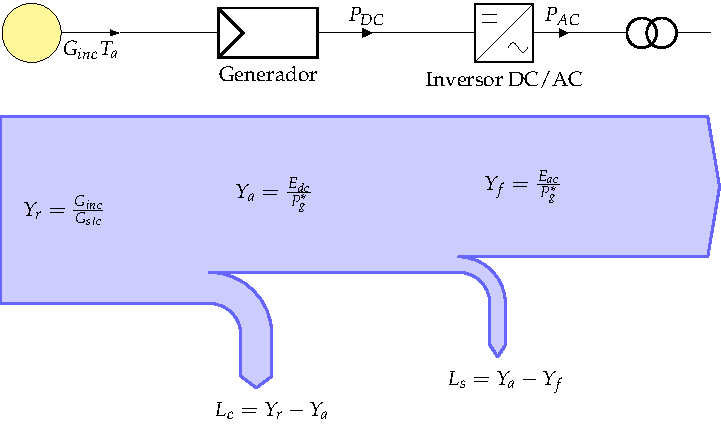
\includegraphics[height=0.9\textheight]{../figs/SankeyDiagrama_SFCR.pdf}
\end{center}
\end{frame}

\section{Métricas de Rendimiento}
\label{sec:org7f4421f}

\begin{frame}[label={sec:org896e582}]{\emph{Performance Ratio} o rendimiento global}
\[
  PR = \frac{Y_f}{Y_r} = \frac{E_{ac}}{P_g^* \cdot \frac{G_{inc}}{G_{stc}}}
\]

\begin{itemize}
\item Está concebido para incluir todas las \alert{pérdidas que no tienen
dependencia con las condiciones meteorológicas}.

\item Este factor \emph{puede} caracterizar el funcionamiento de un sistema
\alert{independientemente de la localidad}.

\item En sentido estricto no es cierto porque sí hay \alert{relación con la temperatura}.

\begin{itemize}
\item Un mismo sistema tendrá un PR más alto en un lugar de clima frío que en un lugar de clima cálido.

\item El PR de un sistema es estacional (más alto en invierno que en verano).
\end{itemize}
\end{itemize}
\end{frame}

\begin{frame}[label={sec:orgf60e272}]{Valores del PR}
\begin{itemize}
\item El análisis de funcionamiento de diversos sistemas FV europeos ha
mostrado que el rango de valores que toma el \emph{performance ratio} es
bastante amplio, con mínimos de 0,4 y máximos de 0,85.

\item Para sistemas instalados entre 1980 a 1990, \alert{el valor promedio ha sido de
0,7}.

\item Para sistemas instalados entre 2005 a 2012, \alert{el valor promedio ha
sido de 0,8}.
\end{itemize}
\end{frame}


\begin{frame}[label={sec:org292cc69}]{Rendimiento Global \(\qty{25}{\celsius}\)}
\[
  PR_{25} = \frac{E_{ac}}{\sum_i \left\{P_g^* \cdot \left[1 + \gamma_P \cdot(T_{c,i} - 25)\right]\cdot G_{ef,i}/G_{stc} \cdot \Delta t \right\}}
\]
\begin{itemize}
\item Se introduce una corrección con la temperatura utilizando el coeficiente \(\gamma\) de dependencia de la potencia del módulo con la temperatura.
\item \(\Delta t\) es el intervalo temporal de medida.
\item No elimina totalmente la dependencia estacional porque hay otros efectos estacionales (sombras).
\end{itemize}
\end{frame}
\end{document}
